\documentclass[aspectratio=169]{beamer}
\usetheme{Madrid}
\usecolortheme{beaver}
\usepackage{booktabs}
\usepackage{hyperref}
\usepackage{tikz}
\usepackage{amsmath}
\usepackage{graphicx}

\title{Expanding the Horizons: ML \& RL Beyond LLMs}
\subtitle{Machine Learning and Reinforcement Learning for Programmers}
\author{Batuhan Başerdem}
\date{\today}

\begin{document}

\frame{\titlepage}

% Slide 1: Title & Overview
\begin{frame}{Overview}
  \begin{itemize}
    \item ML basics and neural architectures
    \item Key ML domains outside of LLMs
    \item Reinforcement learning applications and emerging trends
    \item RL on top of LLMs (RLHF)
    \item Practical integration into real-world codebases
  \end{itemize}
\end{frame}

% Slide 2: What is Machine Learning?
\begin{frame}{What is Machine Learning?}
  \textbf{Definition:} Training systems to learn from data and improve over time

  \vspace{0.5cm}
  \textbf{Key Categories:}
  \begin{itemize}
    \item \textbf{Supervised Learning:} Models learn from labeled data
    \item \textbf{Unsupervised Learning:} Models uncover patterns without labels
    \item \textbf{Reinforcement Learning:} Agents learn by trial and error
  \end{itemize}

  \vspace{0.5cm}
  \textbf{Core Concept:} Generalization from past experience
\end{frame}

% Slide 3: Neural Networks
\begin{frame}{Neural Networks — The Backbone}
  \textbf{Definition:} Computational systems inspired by the human brain

  \vspace{0.3cm}
  \textbf{Functions:}
  \begin{itemize}
    \item Fit nonlinear functions
    \item Recognize patterns
    \item Automate feature extraction
  \end{itemize}

  \vspace{0.3cm}
  \textbf{Modern Architectures:}
  \begin{itemize}
    \item Feedforward Networks
    \item Convolutional Neural Networks (CNNs)
    \item Recurrent Neural Networks (RNNs/LSTMs)
    \item Transformers
  \end{itemize}
\end{frame}

% Slide 4: Types of Neural Net Architectures
\begin{frame}{Types of Neural Net Architectures}
  \begin{table}
    \centering
    \begin{tabular}{ll}
      \toprule
      \textbf{Architecture} & \textbf{Typical Application} \\
      \midrule
      Feedforward NN & Credit scoring, tabular data \\
      CNN (ConvNet) & Image \& video processing \\
      RNN/LSTM & Time series, NLP, speech \\
      Transformers & Language and vision tasks \\
      \bottomrule
    \end{tabular}
  \end{table}

  \vspace{0.5cm}
  Each architecture is specialized for certain data types and tasks
\end{frame}

% Slide 5: ML Beyond LLMs
\begin{frame}{ML Beyond LLMs — Real-World Workhorses}
  \begin{columns}
    \column{0.5\textwidth}
    \textbf{Core Applications:}
    \begin{itemize}
      \item \textbf{Image Processing:} Medical imaging, defect detection
      \item \textbf{Computational Chemistry:} Drug discovery
      \item \textbf{Robotics:} Perception, navigation
      \item \textbf{Anomaly Detection:} Fraud, cybersecurity
      \item \textbf{Automated Driving:} Sensor fusion
    \end{itemize}

    \column{0.5\textwidth}
    \textbf{Other Examples:}
    \begin{itemize}
      \item Time series forecasting
      \item Speech recognition
      \item Recommendation systems
      \item Industrial automation
      \item Energy optimization
    \end{itemize}
  \end{columns}
\end{frame}

% Slide 6: Neural Network Architecture
\begin{frame}{Neural Network Architecture}
  \begin{columns}
    \column{0.55\textwidth}
    \begin{center}
      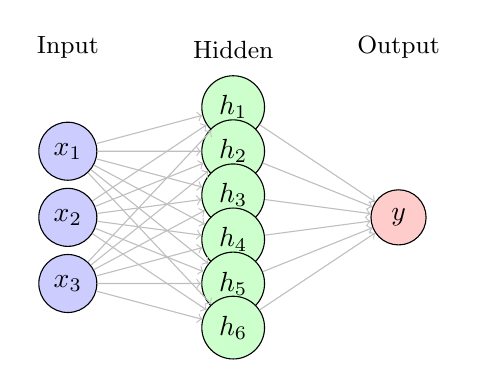
\begin{tikzpicture}[scale=0.7]
        % Input layer
        \foreach \i in {1,2,3} {
          \node[circle, draw, fill=blue!20, minimum size=0.7cm] (input\i) at (0, -\i*1.2) {$x_\i$};
        }
        
        % Hidden layer
        \foreach \j in {1,...,6} {
          \node[circle, draw, fill=green!20, minimum size=0.7cm] (hidden\j) at (3, -\j*0.8 + 0.4) {$h_\j$};
        }
        
        % Output layer
        \node[circle, draw, fill=red!20, minimum size=0.7cm] (output) at (6, -2.4) {$y$};
        
        % Connections from input to hidden
        \foreach \i in {1,2,3} {
          \foreach \j in {1,...,6} {
            \draw[->, gray!50] (input\i) -- (hidden\j);
          }
        }
        
        % Connections from hidden to output
        \foreach \j in {1,...,6} {
          \draw[->, gray!50] (hidden\j) -- (output);
        }
        
        % Labels
        \node[above] at (0, 0.3) {\small Input};
        \node[above] at (3, 0.3) {\small Hidden};
        \node[above] at (6, 0.3) {\small Output};
      \end{tikzpicture}
    \end{center}
    
    \column{0.45\textwidth}
    \textbf{Forward Propagation:}
    \vspace{0.3cm}
    
    \small
    Hidden layer activation:
    $$h_j = f\left(\sum_{i=1}^{3} w_{ij}^{(1)} x_i + b_j^{(1)}\right)$$
    
    \vspace{0.2cm}
    Output layer activation:
    $$y = g\left(\sum_{j=1}^{6} w_{j}^{(2)} h_j + b^{(2)}\right)$$
    
    \vspace{0.2cm}
    where $f$ and $g$ are activation functions
  \end{columns}
\end{frame}

% Slide 7: Why LLMs Don't Cover it All
\begin{frame}{Why LLMs Don't Cover it All}
  \begin{itemize}
    \item \textbf{Vision Tasks:} LLMs can't natively interpret raw images/videos
    \item \textbf{Physical World:} Robotics requires
      spatial/kinematic understanding
    \item \textbf{Domain Science:} Chemistry and biology need
      physics-aware models
    \item \textbf{Real-time Demands:} Critical systems need low
      latency, specialized models
  \end{itemize}

  \vspace{0.5cm}
  \centering
  \textbf{LLMs are powerful, but purpose-built ML models remain irreplaceable}
\end{frame}

% Slide 8: Convolutional Neural Networks (CNNs)
\begin{frame}{Convolutional Neural Networks (CNNs)}
  \begin{columns}
    \column{0.5\textwidth}
    \textbf{Key Concepts:}
    \begin{itemize}
      \item \textbf{Convolution:} Sliding filters detect features
      \item \textbf{Pooling:} Reduces spatial dimensions
      \item \textbf{Feature Maps:} Learned representations
      \item \textbf{Hierarchical Learning:} From edges to objects
    \end{itemize}
    
    \vspace{0.3cm}
    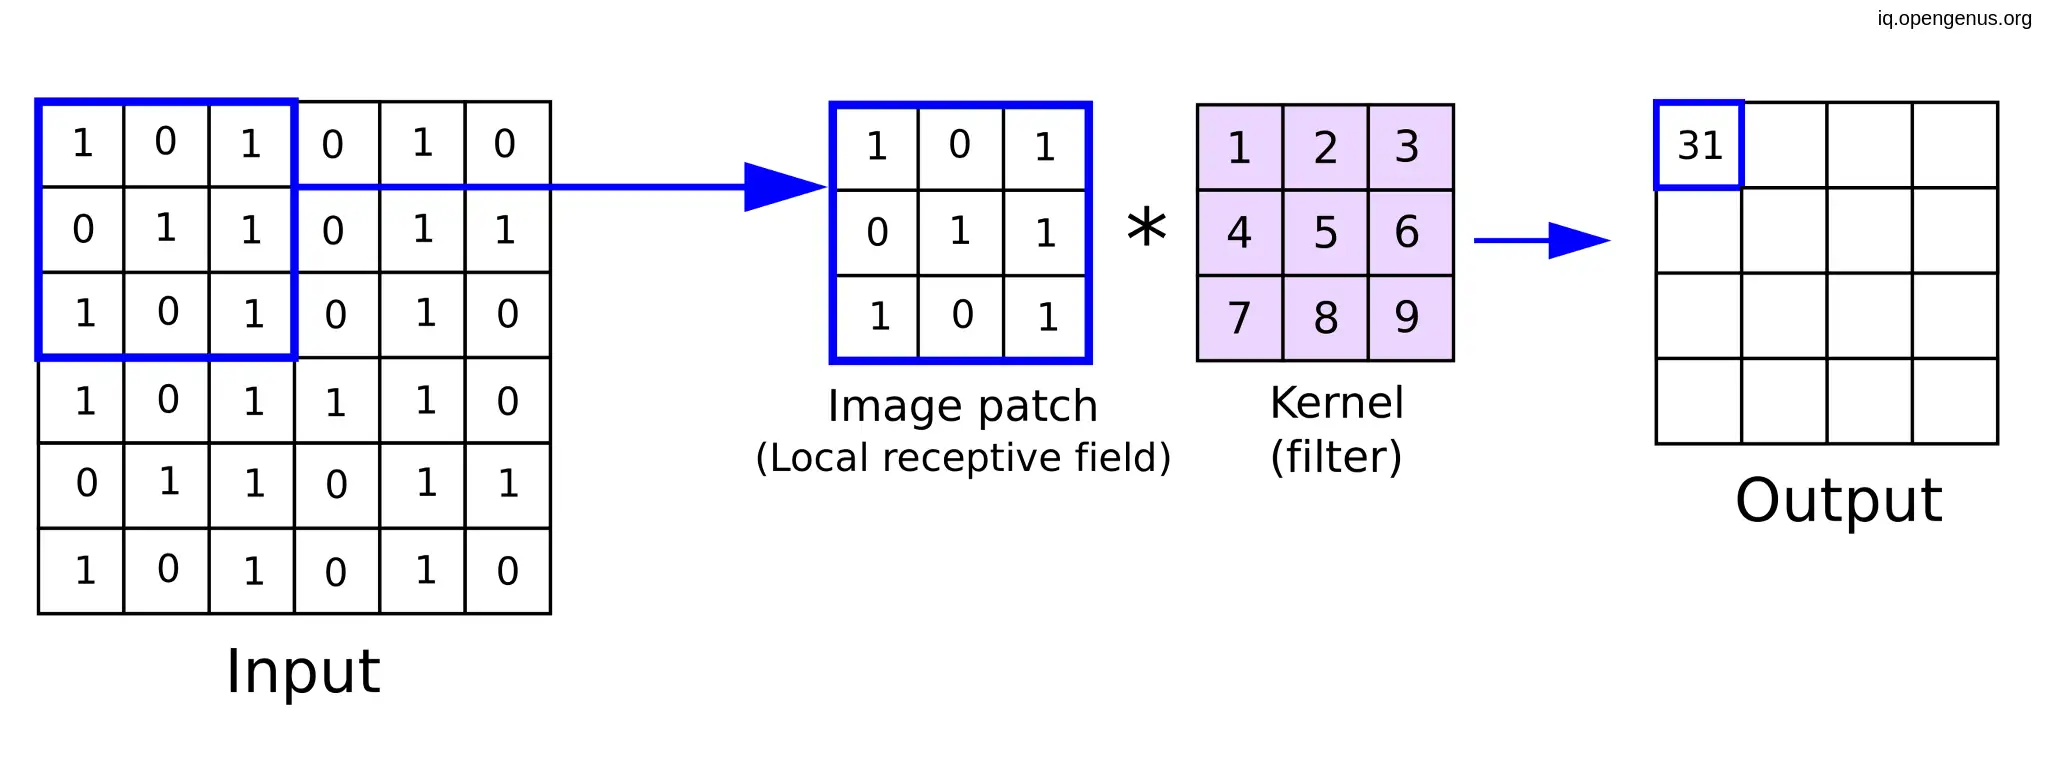
\includegraphics[width=\textwidth]{images/convolutional_layer.png}
    
    \column{0.5\textwidth}
    \textbf{CNN Architecture Example:}
    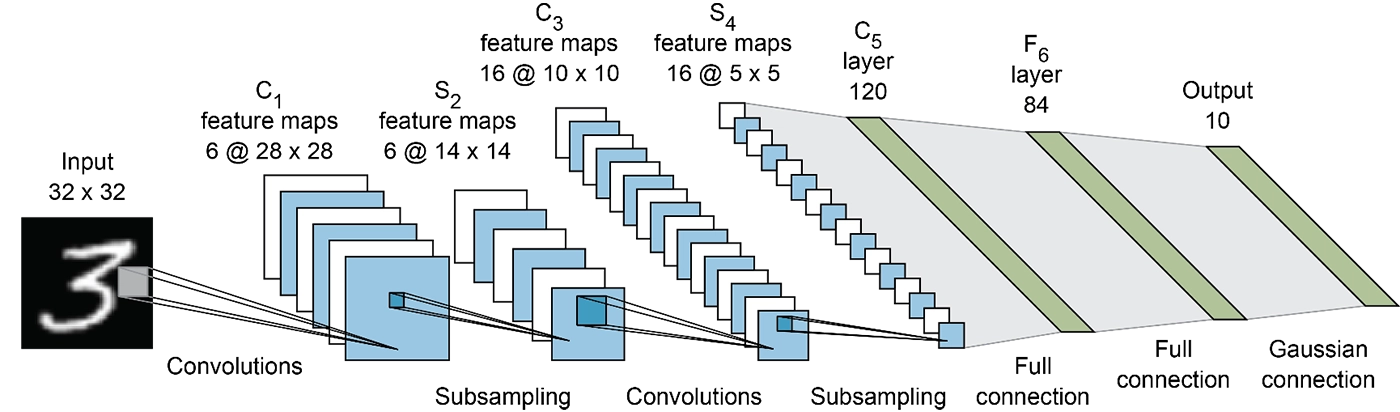
\includegraphics[width=\textwidth]{images/imagenet_architecture.png}
    
    \vspace{0.3cm}
    \textbf{Applications:}
    \begin{itemize}
      \item Image classification
      \item Object detection
      \item Medical imaging
      \item Video analysis
    \end{itemize}
  \end{columns}
\end{frame}

% Slide 9: Encoder-Decoder Architectures
\begin{frame}{Encoder-Decoder Architectures}
  \begin{columns}
    \column{0.45\textwidth}
    \begin{center}
      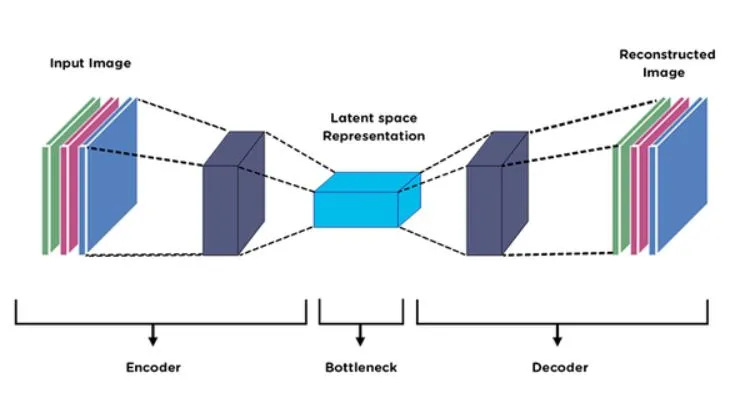
\includegraphics[width=\textwidth]{images/encoderDecoder.png}
    \end{center}
    
    \vspace{0.3cm}
    \textbf{Key Components:}
    \small
    \begin{itemize}
      \item \textbf{Encoder:} Compresses input
      \item \textbf{Bottleneck:} Latent space
      \item \textbf{Decoder:} Reconstructs output
    \end{itemize}
    
    \column{0.55\textwidth}
    \textbf{Applications:}
    \begin{itemize}
      \item \textbf{Autoencoders:} Data compression, denoising
      \item \textbf{VAEs:} Generative modeling
      \item \textbf{Seq2Seq:} Machine translation
      \item \textbf{U-Net:} Image segmentation
      \item \textbf{BERT:} Bidirectional encoding
    \end{itemize}
    
    \vspace{0.3cm}
    \textbf{Key Insight:} Learn meaningful representations by forcing information through a bottleneck
  \end{columns}
\end{frame}

% Slide 10: Generative Adversarial Networks (GANs)
\begin{frame}{Generative Adversarial Networks (GANs)}
  \begin{columns}
    \column{0.5\textwidth}
    \begin{center}
      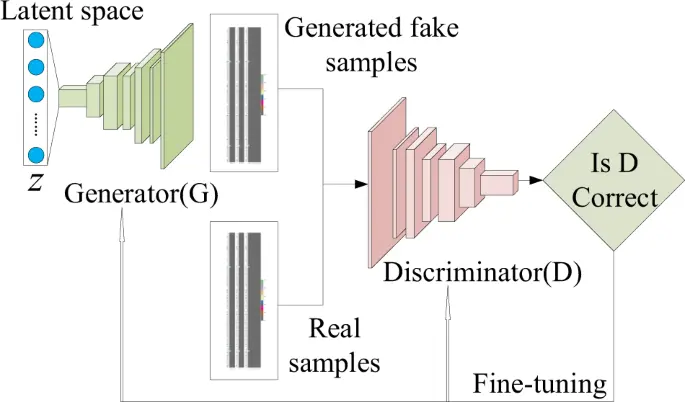
\includegraphics[width=\textwidth]{images/gan.png}
    \end{center}
    
    \textbf{Two-Player Game:}
    \small
    \begin{itemize}
      \item \textbf{Generator:} Creates fake samples
      \item \textbf{Discriminator:} Real vs fake
      \item \textbf{Adversarial:} Compete to improve
    \end{itemize}
    
    \column{0.5\textwidth}
    \textbf{Applications:}
    \begin{itemize}
      \item \textbf{Image Generation:} DALL-E, Midjourney
      \item \textbf{Style Transfer:} Artistic rendering
      \item \textbf{Data Augmentation:} Training data
      \item \textbf{Super-resolution:} Image enhancement
      \item \textbf{Video Synthesis:} Deepfakes
    \end{itemize}
    
    \vspace{0.2cm}
    \textbf{Key Insight:} Competition drives both networks to improve
  \end{columns}
\end{frame}

% Transition Slide: From ML to RL
\begin{frame}[plain]
  \begin{center}
    \vspace{2cm}
    \Huge\textbf{Reinforcement Learning}
    
    \vspace{1cm}
    \Large Learning Through Interaction
    
    \vspace{2cm}
    \normalsize From Pattern Recognition to Decision Making
  \end{center}
\end{frame}

% Slide 11: What is Reinforcement Learning?
\begin{frame}{What is Reinforcement Learning (RL)?}
  \textbf{Core Idea:} Agent explores, makes decisions, receives
  rewards/punishments

  \vspace{0.5cm}
  \begin{center}
    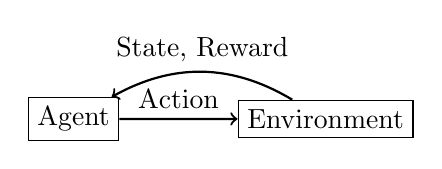
\begin{tikzpicture}[scale=0.8]
      \node[draw, rectangle] (agent) at (0,2) {Agent};
      \node[draw, rectangle] (env) at (4,2) {Environment};
      \draw[->, thick] (agent) -- node[above] {Action} (env);
      \draw[->, thick] (env) to[bend right=30] node[above] {State, Reward} (agent);
    \end{tikzpicture}
  \end{center}

  \vspace{0.5cm}
  \textbf{Distinction:} Not about predicting outputs, but learning
  sequential decision policies
\end{frame}

% Slide 8: RL Concepts
\begin{frame}{RL Concepts Key to Practitioners}
  \begin{columns}
    \column{0.5\textwidth}
    \textbf{Core Components:}
    \begin{itemize}
      \item \textbf{Agent:} The decision maker
      \item \textbf{Environment:} Where agent acts
      \item \textbf{State:} Current situation
      \item \textbf{Action:} Available choices
      \item \textbf{Reward:} Feedback signal
    \end{itemize}

    \column{0.5\textwidth}
    \textbf{Key Concepts:}
    \begin{itemize}
      \item \textbf{Policy:} How to act in each state
      \item \textbf{Reward Function:} Quantifies feedback
      \item \textbf{Exploration vs. Exploitation:} Balancing new
        trials and established actions
    \end{itemize}
  \end{columns}
\end{frame}

% Slide: Value and Q Functions Part 1
\begin{frame}{Value Functions: Policy and State Values}
  \textbf{Policy $\pi$:} Defines the agent's behavior
  \begin{center}
    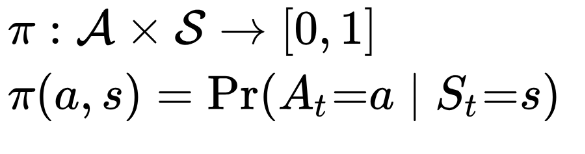
\includegraphics[width=0.4\textwidth]{images/policy.png}
  \end{center}
  
  \vspace{0.5cm}
  \textbf{State-Value Function $V^\pi(s)$:} Expected return starting from state $s$ following policy $\pi$
  \begin{center}
    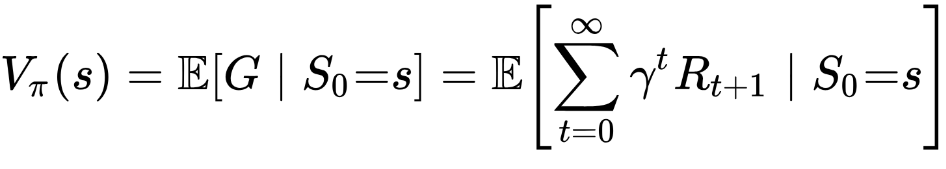
\includegraphics[width=0.7\textwidth]{images/valuefunct.png}
  \end{center}
\end{frame}

% Slide: Value and Q Functions Part 2
\begin{frame}{Value Functions: Action Values}
  \textbf{Action-Value Function $Q^\pi(s,a)$:} Expected return starting from state $s$, taking action $a$, then following policy $\pi$
  
  \vspace{0.5cm}
  \begin{center}
    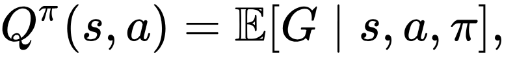
\includegraphics[width=0.6\textwidth]{images/qvalue.png}
  \end{center}
  
  \vspace{0.5cm}
  \textbf{Key Insight:}
  \begin{itemize}
    \item $V^\pi(s)$ tells us how good a state is
    \item $Q^\pi(s,a)$ tells us how good an action is in a given state
    \item Both depend on the policy $\pi$ being followed
  \end{itemize}
\end{frame}

% Slide: Example Trajectories
\begin{frame}{Example Trajectories with Different Discount Factors}
  \begin{columns}
    \column{0.5\textwidth}
    \begin{center}
      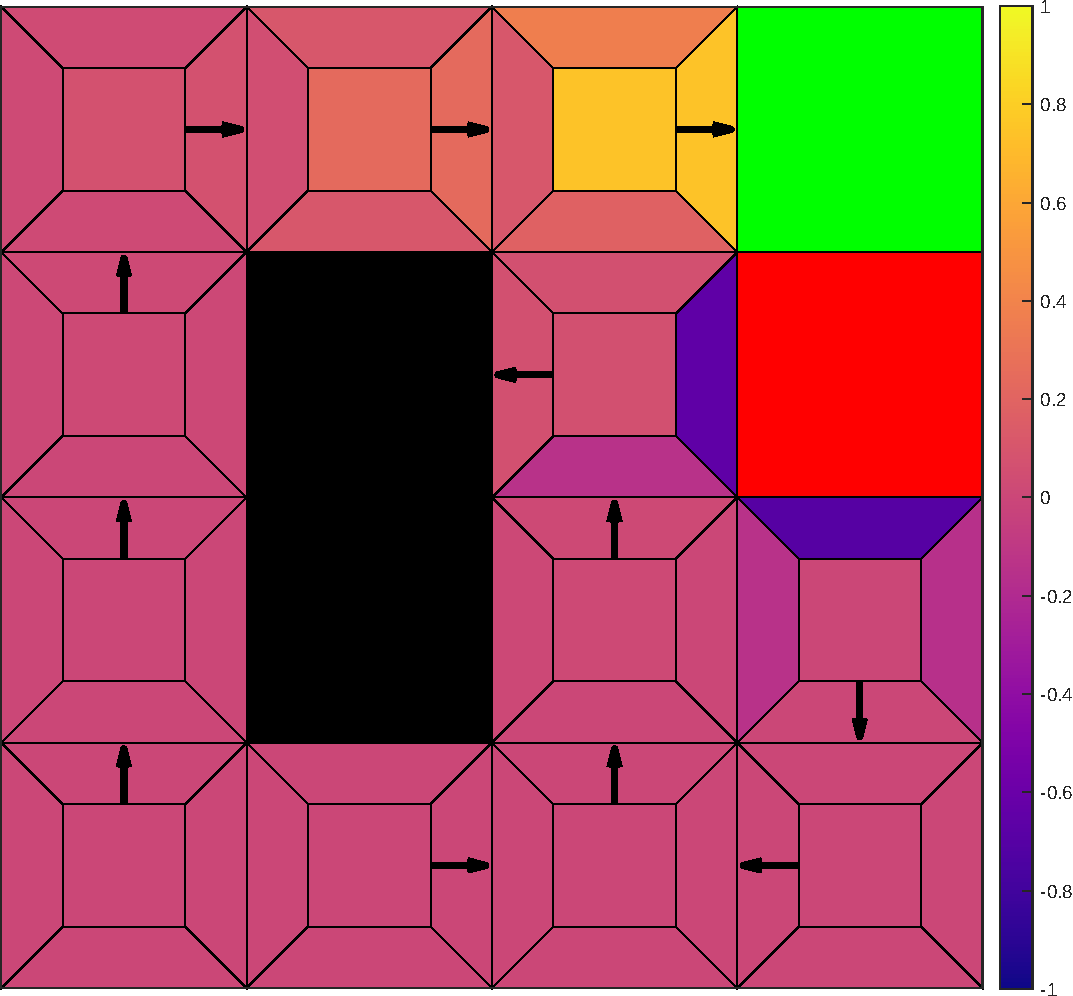
\includegraphics[width=\textwidth]{images/ex_gam4-eps-converted-to.pdf}
      
      \textbf{$\gamma = 0.4$}
    \end{center}
    
    \column{0.5\textwidth}
    \begin{center}
      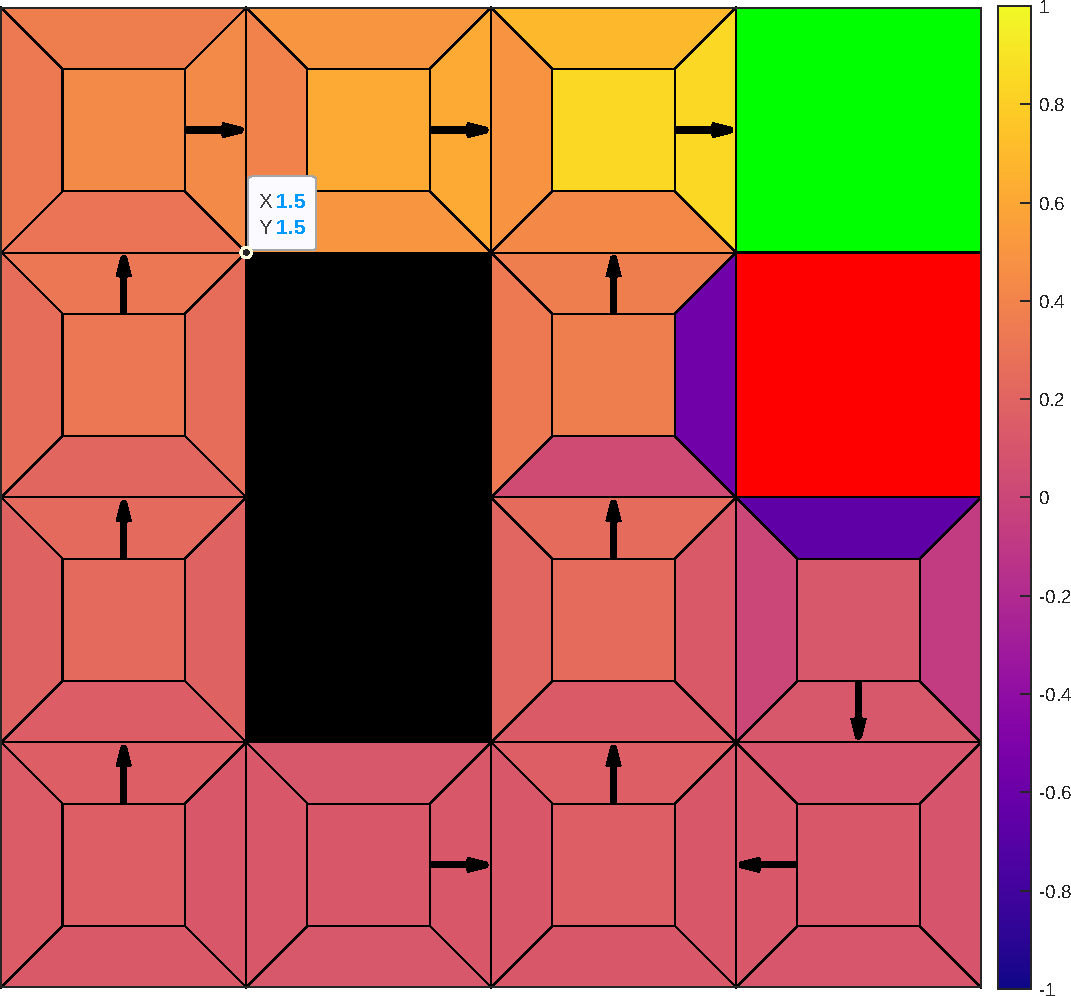
\includegraphics[width=\textwidth]{images/ex_gam8-eps-converted-to.pdf}
      
      \textbf{$\gamma = 0.8$}
    \end{center}
  \end{columns}
  
  \vspace{0.5cm}
  \textbf{Discount Factor Impact:}
  \begin{itemize}
    \item Lower $\gamma$: Focus on immediate rewards
    \item Higher $\gamma$: Consider long-term rewards
  \end{itemize}
\end{frame}

% Slide 12: RL in Practice
\begin{frame}{RL in Practice — Beyond LLMs}
  \begin{columns}
    \column{0.5\textwidth}
    \textbf{Classic Domains:}
    \begin{itemize}
      \item Robotics (navigation, manipulation)
      \item Automated Driving
      \item Games (chess, Go, e-sports)
      \item Industrial Automation
    \end{itemize}

    \column{0.5\textwidth}
    \textbf{Emerging Domains:}
    \begin{itemize}
      \item Healthcare: Treatment optimization
      \item Finance: Algorithmic trading
      \item Energy: Smart grid, HVAC
      \item Networking: Resource scheduling
    \end{itemize}
  \end{columns}

  \vspace{0.5cm}
  \centering
  \textbf{RL is increasingly practical with better simulators and frameworks}
\end{frame}

% Slide: Actor-Critic Architecture
\begin{frame}{Actor-Critic: Combining Policy and Value}
  \begin{columns}
    \column{0.5\textwidth}
    \begin{center}
      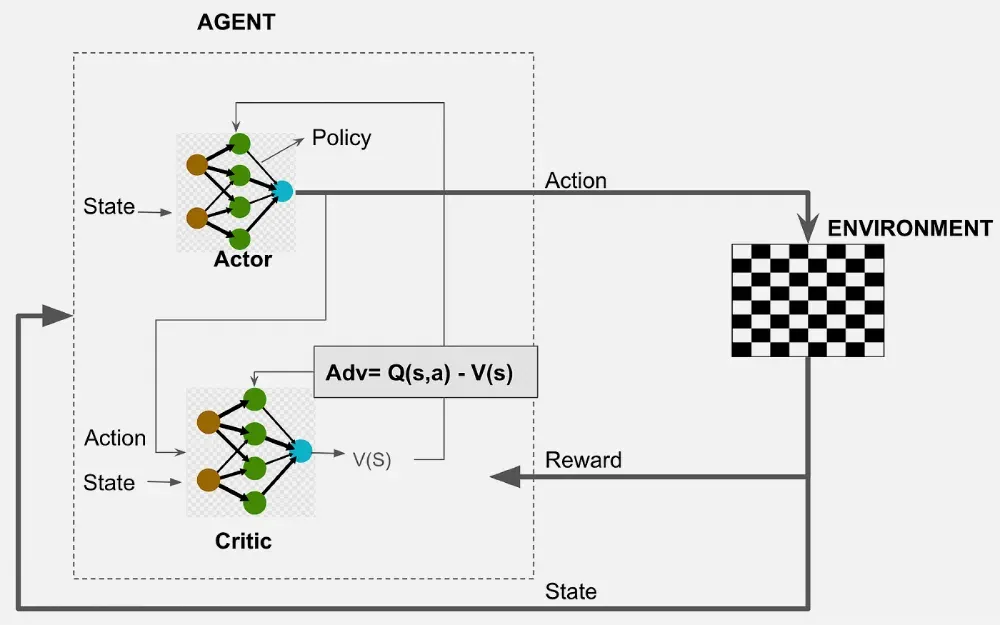
\includegraphics[width=\textwidth]{images/actorcritic.png}
    \end{center}
    
    \column{0.5\textwidth}
    \textbf{Two Neural Networks:}
    \begin{itemize}
      \item \textbf{Actor:} Learns the policy $\pi(a|s)$
      \item \textbf{Critic:} Learns the value function $V(s)$
    \end{itemize}
    
    \vspace{0.5cm}
    \textbf{Key Benefits:}
    \begin{itemize}
      \item More stable than pure policy gradient
      \item Reduces variance in learning
      \item Foundation for modern algorithms (A3C, PPO, SAC)
    \end{itemize}
  \end{columns}
\end{frame}

% Slide 10: RL's Current Frontier
\begin{frame}{RL's Current Frontier}
  \begin{itemize}
    \item \textbf{Hybrid Learning:} Mixing RL with
      supervised/unsupervised learning
    \item \textbf{Sample Efficiency:} Model-based RL, offline RL for
      less real-world data
    \item \textbf{Transfer Learning:} Skills from simulation to real world
    \item \textbf{Safety and Ethics:} Constrained RL for critical systems
  \end{itemize}

  \vspace{0.5cm}
  \centering
  Focus on making RL more practical and deployable
\end{frame}

% Slide: RLHF Process Overview
\begin{frame}{RLHF Process Overview}
  \begin{center}
    \resizebox{0.9\textwidth}{!}{
    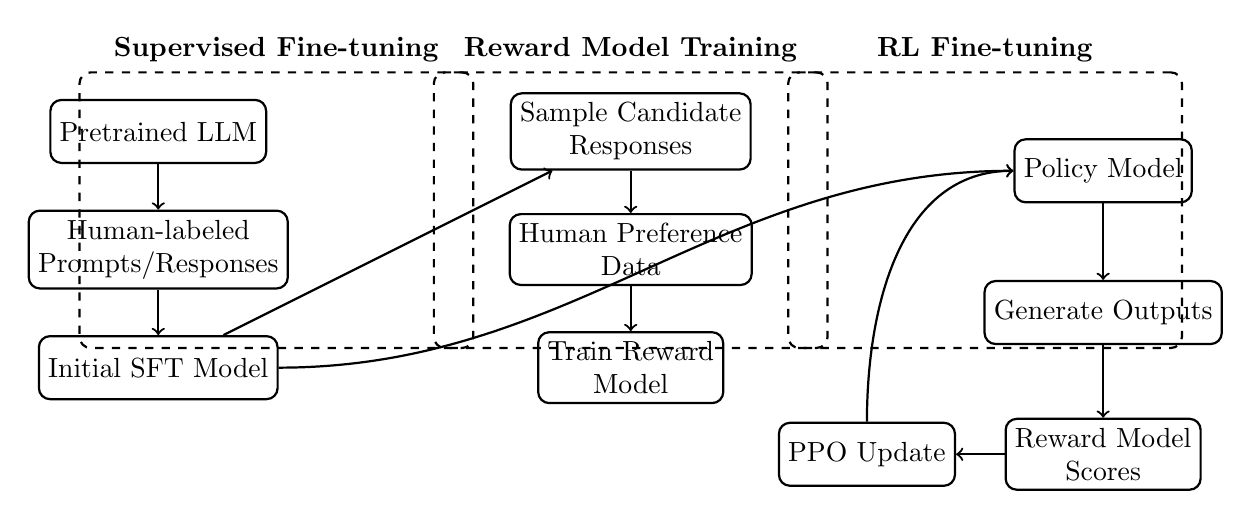
\begin{tikzpicture}[
      node distance=1.5cm and 2cm,
      box/.style={rectangle, draw, thick, minimum height=0.8cm, align=center, rounded corners},
      group/.style={rectangle, draw, dashed, thick, rounded corners}
    ]
      % SFT Group
      \node[group, minimum width=5cm, minimum height=3.5cm] (sft_group) {};
      \node[above] at (sft_group.north) {\textbf{Supervised Fine-tuning}};
      
      \node[box] (pretrained) at (-1.5, 1) {Pretrained LLM};
      \node[box, below of=pretrained] (human_data) {Human-labeled\\Prompts/Responses};
      \node[box, below of=human_data] (sft_model) {Initial SFT Model};
      
      \draw[->, thick] (pretrained) -- (human_data);
      \draw[->, thick] (human_data) -- (sft_model);
      
      % Reward Model Group
      \node[group, minimum width=5cm, minimum height=3.5cm, right of=sft_group, xshift=3cm] (reward_group) {};
      \node[above] at (reward_group.north) {\textbf{Reward Model Training}};
      
      \node[box] (sample) at (4.5, 1) {Sample Candidate\\Responses};
      \node[box, below of=sample] (pref_data) {Human Preference\\Data};
      \node[box, below of=pref_data] (train_reward) {Train Reward\\Model};
      
      \draw[->, thick] (sft_model) -- (sample);
      \draw[->, thick] (sample) -- (pref_data);
      \draw[->, thick] (pref_data) -- (train_reward);
      
      % RL Group
      \node[group, minimum width=5cm, minimum height=3.5cm, right of=reward_group, xshift=3cm] (rl_group) {};
      \node[above] at (rl_group.north) {\textbf{RL Fine-tuning}};
      
      \node[box] (policy) at (10.5, 0.5) {Policy Model};
      \node[box, below of=policy, yshift=-0.3cm] (generate) {Generate Outputs};
      \node[box, below of=generate, yshift=-0.3cm] (scores) {Reward Model\\Scores};
      \node[box, left of=scores, xshift=-1.5cm] (ppo) {PPO Update};
      
      \draw[->, thick] (sft_model) to[out=0,in=180] (policy);
      \draw[->, thick] (policy) -- (generate);
      \draw[->, thick] (generate) -- (scores);
      \draw[->, thick] (scores) -- (ppo);
      \draw[->, thick] (ppo) to[out=90,in=180] (policy);
    \end{tikzpicture}
    }
  \end{center}
\end{frame}

% Slide 11: RLHF
\begin{frame}{Deep Dive — RL on Top of LLMs (RLHF)}
  \textbf{RLHF (Reinforcement Learning from Human Feedback):}
  \begin{itemize}
    \item Combines RL with human ratings to refine LLM outputs
    \item Example: ChatGPT, GPT-4 use RLHF for alignment
  \end{itemize}

  \vspace{0.3cm}
  \textbf{Process:}
  \begin{enumerate}
    \item Human evaluators rank outputs
    \item Model learns a reward function
    \item RL fine-tunes model to maximize predicted human reward
  \end{enumerate}

  \vspace{0.3cm}
  \textbf{Benefits:} Safer, more aligned, less toxic responses\\
  \textbf{Challenges:} Scaling human feedback, addressing evaluator bias
\end{frame}

% Slide 12: RLHF State of the Art
\begin{frame}{RLHF — State of the Art and Beyond}
  \textbf{Techniques:}
  \begin{itemize}
    \item Direct Preference Optimization (DPO)
    \item Safe RLHF
    \item Reward modeling from human and AI sources
  \end{itemize}

  \vspace{0.3cm}
  \textbf{Emerging Frameworks:}
  \begin{itemize}
    \item Open source RLHF libraries (e.g., OpenRLHF)
    \item Streamlined model fine-tuning for LLMs
  \end{itemize}

  \vspace{0.3cm}
  \textbf{Research Directions:}
  \begin{itemize}
    \item Personalized reward models
    \item RLHF for computer vision and robotics
    \item Multi-modal agents
  \end{itemize}
\end{frame}

% Slide 13: RLHF in Open-source Agents
\begin{frame}{RLHF in Open-source Agents}
  \textbf{Example: Ruler (OpenPipe)}
  \begin{itemize}
    \item Integrates LLMs, tools, memory, and RLHF-style feedback
    \item Creates fully automated, interactive software agents
  \end{itemize}

  \vspace{0.5cm}
  \textbf{Implications:}
  \begin{itemize}
    \item Agents that learn from users in real deployments
    \item Adapt tool use based on feedback
    \item Align to organizational values with less manual rule-setting
  \end{itemize}

  \vspace{0.5cm}
  \centering
  \textbf{RL/RLHF paradigm is moving from research to practical frameworks}
\end{frame}

% Slide 14: Resources
\begin{frame}{Resources \& Deeper Dives}
  \textbf{Online Courses/Books:}
  \begin{itemize}
    \item Coursera, edX courses
    \item NeurIPS/ICML tutorials
  \end{itemize}

  \vspace{0.3cm}
  \textbf{Practical RL Frameworks:}
  \begin{itemize}
    \item Stable Baselines3
    \item RLlib
    \item OpenRLHF
  \end{itemize}

  \vspace{0.3cm}
  \textbf{Further Reading:}
  \begin{itemize}
    \item Recent reviews on RLHF and RL frontiers
    \item State-of-the-art trends and practical challenges
  \end{itemize}
\end{frame}

% Slide 15: Q&A
\begin{frame}{Q\&A and Discussion}
  \centering
  \Large
  Questions about:
  \begin{itemize}
    \item Practical deployment?
    \item RL/RLHF challenges?
    \item ML use cases?
    \item Getting started with these frameworks?
  \end{itemize}
\end{frame}

% Thank You Slide
\begin{frame}[plain]
  \begin{center}
    \vspace{3cm}
    \Huge\textbf{Thank You for Listening!}
    
    \vspace{2cm}
    \Large Questions \& Discussion
  \end{center}
\end{frame}

\end{document}

